\begin{figure}[tbp]
\centering
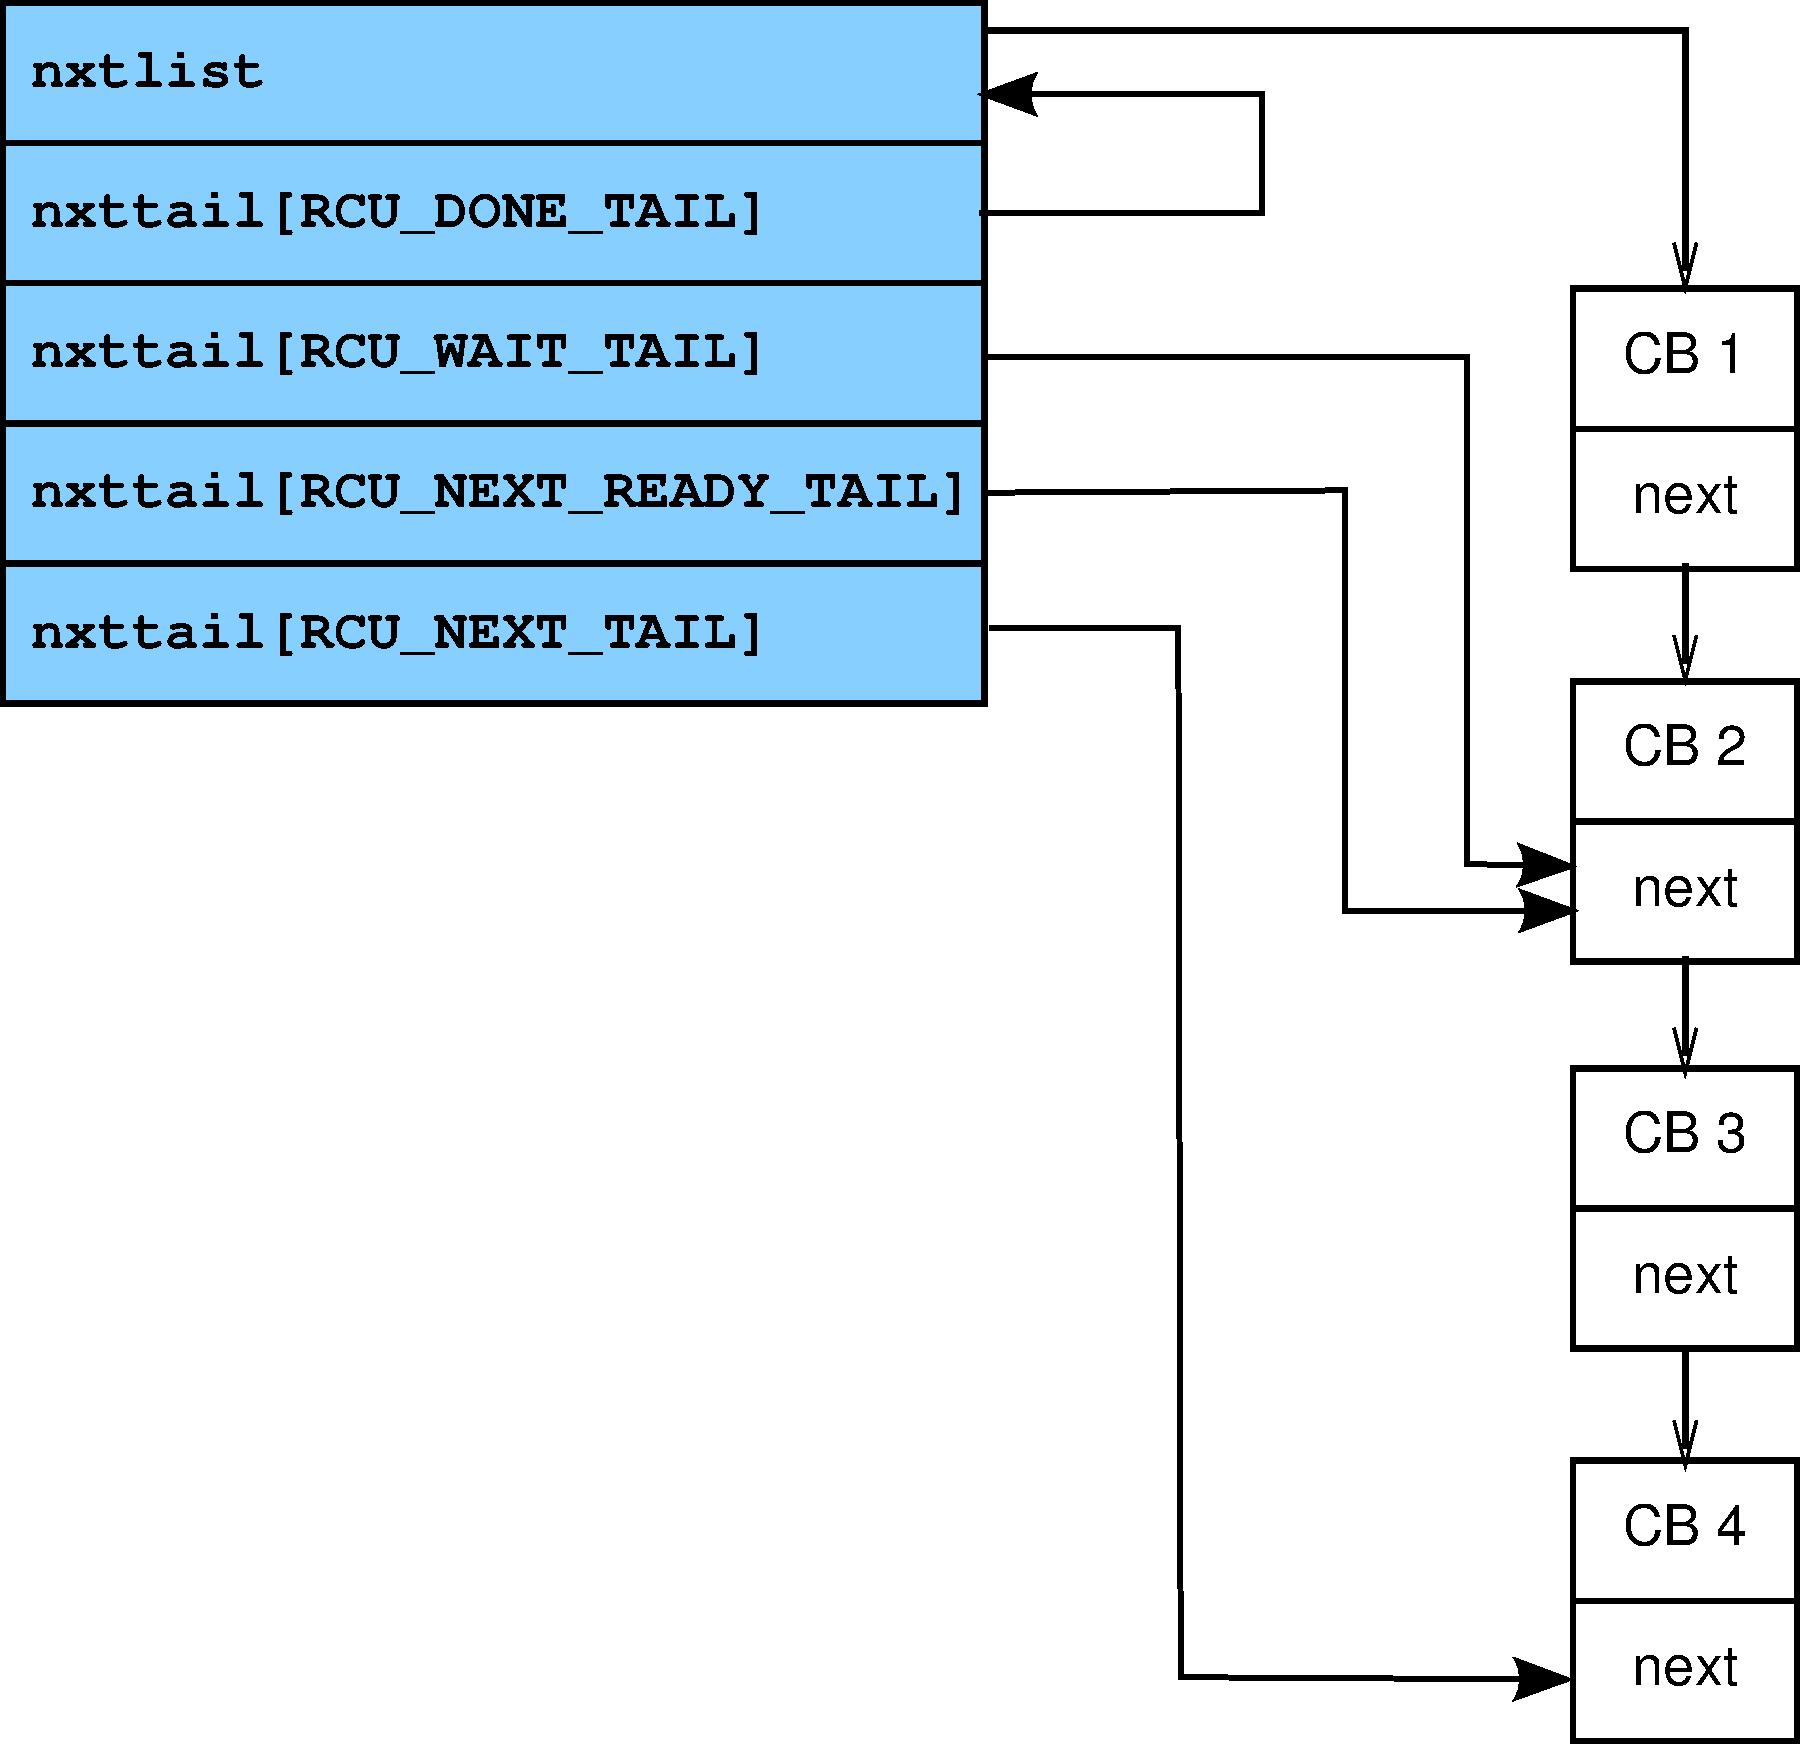
\includegraphics[scale=0.25]{rcu_data_callbacks.pdf}
\caption{Callback Queuing in \co{rcu_data}}
\label{fig:rcu_data_callbacks}
\end{figure}

%\comment{Lihao: since we don't model callbacks, only describe them briefly and add a reference
%to save space for the experiments section which is the main contribution of this paper. 
%Do the same for discussion of preemptible RCU.}
\subsubsection{RCU Callbacks}
The \co{rcu_data} structure manages RCU callbacks using a \co{->nxtlist}
pointer tracking the head of the list and an array of \co{->nxttail[]}
tail pointers that form a four-segment list of
callbacks~\cite{LaiJiangshan2008NewClassicAlgorithm}, with
each element of the \co{->nxttail[]} array referencing the tail of the
corresponding segment, as shown in Figure~\ref{fig:rcu_data_callbacks}.
The segment ending with \co{->nxttail[RCU_DONE_TAIL]} (the ``\co{RCU_DONE_TAIL}
segment'') contains callbacks
handled by a prior grace period that are therefore ready to be invoked.
The \co{RCU_WAIT_TAIL} and \co{RCU_NEXT_READY_TAIL} segments 
contain callbacks waiting for the
current and the next grace period, respectively.
Finally, the \co{RCU_NEXT_TAIL} segment contains
callbacks that are not yet associated with any grace period.
%
The \co{->qlen} field counts the total number of callbacks, and
the \co{->blimit} field specifies the maximum number of RCU callbacks
that may be invoked at a given time, thus limiting response-time
degradation due to long lists of callbacks.\footnote{
	Workloads requiring aggressive real-time guarantees should use
	callback offloading, which is outside of the scope of this paper.}

Back in Figure~\ref{fig:rcu_data_callbacks}, the
\co{->nxttail[RCU_DONE_TAIL]} array element references \co{->nxtlist}, 
which means none of the callbacks are ready to invoke.
The \co{->nxttail[RCU_WAIT_TAIL]} element references callback 2's \co{->next}
pointer, meaning that callbacks CB~1 and CB~2 are waiting for the current
grace period.
The \co{->nxttail[RCU_NEXT_READY_TAIL]} element references that same \co{->next}
pointer, meaning that no callbacks are waiting for the next grace period. 
Finally, the callbacks between the \co{->nxttail[RCU_NEXT_READY_TAIL]} and
\co{->nxttail[RCU_NEXT_TAIL]} elements (CB~3 and CB~4)
are not yet assigned to a specific grace period.
The \co{->nxttail[RCU_NEXT_TAIL]} element always references either
the last callback or, when the entire list is empty, \co{->nxtlist}.

Cache locality is promoted by invoking callbacks on the CPU that registered
them.
For example, RCU's update-side primitive 
\co{synchronize_rcu()} appends callback \co{wakeme_after_rcu()} to the end
of the \co{->nxttail[RCU_NEXT_TAIL]} list in the current CPU 
(Section \ref{sec:update_api_impl}). 
They are advanced one segment towards the head of the list (via \co{rcu_advance_cbs()}) 
when the CPU detects the current grace period has ended, which is indicated 
by the \co{->completed} field of the CPU's \co{rcu_data} structure being one
smaller than its counterpart in the corresponding leaf \co{rcu_node} structure.
The CPU also periodically merges the \co{RCU_NEXT_TAIL} segment into the
\co{RCU_NEXT_READY_TAIL} segment by calling \co{rcu_accelerate_cbs()}.
In a few special cases, the CPU merges the \co{RCU_NEXT_TAIL} segment
into the \co{RCU_WAIT_TAIL} segment, bypassing the \co{RCU_NEXT_TAIL}
segment.
This optimization applies when the CPU is starting a new grace period.
It does \emph{not} apply when a CPU notices a new grace period
because that grace period might well have started before
the callbacks were added to the \co{RCU_NEXT_TAIL} segment.
%\comment{Lihao: why can't we invoke *all* callbacks when starting a new 
%grace period? Isn't it true that all pre-existing read-side critical
%sections, i.e.~those start before callbacks are registered in \co{->nxttail} 
%(in particular \co{wakeme_after_rcu} in \co{->nxttail[RCU_NEXT_TAIL]}), 
%have finished?}
%\comment{Paul: In theory, we could, but in practice doing this would
%have several disadvantages:
%(1) All callbacks would be invoked by the grace-period kthread, and
%large systems could generate more callbacks than a single CPU could
%keep up with, which would delay subsequent grace periods and possibly
%even run the system out of memory.
%(2) Running all the callbacks at once could degrade real-time response.
%(3) Running callbacks on a different CPU than the one that registered
%them would decrease locality, increasing cache-miss rates, thus degrading
%performance.
%(4) This would require that atomic instructions be used when registering
%callbacks (as they are for no-CBs CPUs), further degrading performance.
%In addition, we could only invoke callbacks in the \co{RCU_NEXT_TAIL}
%segment, because callbacks in the later segments
%(\co{RCU_NEXT_READY_TAIL}, \co{RCU_WAIT_TAIL}, and
%\co{RCU_DONE_TAIL} might well have been queued \emph{after} the
%recently-completed grace period started.}
%
This is a deliberate design choice: It is more important for the CPUs
to operate independently (thus avoiding contention and synchronization
overhead) than it is to decrease grace-period latencies.
In those rare occasions where low grace-period latency is important,
the \co{synchronize_rcu_expedited()} should be used.
This function has the same semantics as does \co{synchronize_rcu()},
but trades off efficiency optimizations in favor of reduced latency.
% Lihao: this is where the callback of RCU's update API register? 
% Paul: Yes, call_rcu() appends the callback to the end of the current
% CPU's RCU_NEXT_TAIL list.  Ignoring callback offloading for the moment.
% Lihao: we don't model QS forcing and offline CPUs
% Paul: Nor are you modeling callback offloading.  Which is fine, just calling
% it out.  ;-)

Each RCU callbacks is an \co{rcu_head} structure which has a
\co{->next} field that points to the next callback on the list and
a \co{->func} field that references the function to be invoked at the
end of an upcoming grace period.


